\documentclass[11pt]{article} 

\usepackage[utf8]{inputenc} % set input encoding (not needed with XeLaTeX)
\usepackage[margin = 1in]{geometry} % to change the page dimensions
\geometry{a4paper} % or letterpaper (US) or a5paper or....

\usepackage{graphicx} % support the \includegraphics command and options

% \usepackage[parfill]{parskip} % Activate to begin paragraphs with an empty line rather than an indent

%%% PACKAGES
\usepackage{booktabs} % for much better looking tables
\usepackage{array} % for better arrays (eg matrices) in maths
\usepackage{paralist} % very flexible & customisable lists (eg. enumerate/itemize, etc.)
\usepackage{verbatim} % adds environment for commenting out blocks of text & for better verbatim
\usepackage{subfig} % make it possible to include more than one captioned figure/table in a single float
\usepackage{natbib}
\usepackage{amsmath}

\usepackage{fancyhdr} % This should be set AFTER setting up the page geometry
\pagestyle{fancy} % options: empty , plain , fancy
\renewcommand{\headrulewidth}{0pt} % customise the layout...
\lhead{}\chead{}\rhead{}
\lfoot{}\cfoot{\thepage}\rfoot{}

%%% SECTION TITLE APPEARANCE
%\usepackage{sectsty}
\usepackage{tikz}

%%% ToC (table of contents) APPEARANCE
\usepackage[nottoc,notlof,notlot]{tocbibind} % Put the bibliography in the ToC
\usepackage[titles,subfigure]{tocloft} % Alter the style of the Table of Contents

%\allsectionsfont{\sffamily\mdseries\upshape} % (See the fntguide.pdf for font help)
\usepackage{algpseudocode}
\usepackage[lined,commentsnumbered]{algorithm2e}  
\usepackage{color}
\usepackage{listings}
\usepackage{graphicx}
                                

\title{Two Stage Adaptive Design for Prognostic Biomarker Signature with Survival Outcome}
%\author{Biyue Dai}

\begin{document}
\maketitle

%%%%%%%%%%%%%%%%%%%%%%%%%%%%%%%%%%
%%%%%%%%%%%%%%%%%%%%%%%%%%%%%%%%%%
%%%%%%%%%%%%%%%%%%%%%%%%%%%%%%%%%%

\section{Introduction}
	
	\begin{itemize}	
		\item motivation of extending to survival outcomes
		\item overview of methods proposed in this paper
		\item outline of the paper
	\end{itemize}

%%%%%%%%%%%%%%%%%%%%%%%%%%%%%%%%%%
%%%%%%%%%%%%%%%%%%%%%%%%%%%%%%%%%%
%%%%%%%%%%%%%%%%%%%%%%%%%%%%%%%%%%

\section{Methods}	

%%%%%%%%%%%%%%%%%%%%%%%%%%%%%%%%%%
%%%% this section mainly talk about Cross-validated Harrell's C
	\par This Section is devoted to introducing notations and the framework of predicting patients' time-to-event outcome with a prognostic signature or a set of biomarkers. Suppose there are n observations in the data set. For each observation i = 1, ... n, $(T_{i}, \delta_{i})$ is used to denote the survival outcome of the ith observation. $\delta_{i}$ is an indicator that denotes whether an event is observed or not. When $\delta_{i}$ = 1, an event is observed at $T_{i}$. When $\delta_{i} = 0$, the event is censored at $T_{i}$. Under right censoring, this means $T_{i}$ is the event-free period and the actual event occurs at a time point that is after $T_{i}$. There are also p numbers of covariates collected for each observation i. We use X to denote the $n\times p$ covariate matrix. In clinical studies, the time-to-event outcome could be time until patients' death or time until the progression of a disease. Covariates X may include demographical information, molecular biomarkers etc. In this paper, we only consider $n > p$ scenarios.  
%(Biyue needs Mei's help here). 
	
	\par A predictor $\underline{\eta}$ can be built based on covariates X, which could be used to predict the survival outcome. For each observation i, there is a corresponding $\eta_{i}$. In the context of biomarker studies, X can be a set of biomarkers and $\eta$ can be a predictive signature that is built from multiple biomarkers, using any kind of statistical models for survival outcome such as Cox regression, Weibull regression, or non-linear models such as survival random forest. In this paper, we only consider Cox regression, one of the most commonly used models for survival outcome. Cox regression is a semiparametric model based on hazard, which is the rate of event occurance. Under Cox regression, $\eta = X\hat{\beta}$, where $\hat{\beta}$ is the coefficients estimated from the model and $\eta$ itself is the linear predictor\citep{Cox}. Greater $\eta$ means greater hazard or risk and predicts a shorter time until the event happens.	

	\par Suppose a predictor $\eta$ has already been built, one wants to evaluate its predictive accuarcy. Unlike continuous outcome and binary outcome, there is no obvious way to do this for survival outcome. Van Houwelingen and Putty gave a good summary of works that have been done in this area \citep{Houwelingen2011}. The problem gets more complicated if the validation procedure is not external. If the same data is used to build and evaluate the predictor, then the results would tend to have an optimistic bias. Resampling methods such as cross-validation are commonly used for continuous or binary outcomes. However, cross-validation is not straightforward for survival data, especially for predictors built from Cox regression, where the baseline hazard is not estimated from the model. In the rest of this section, we will introduce a framework where the cross-validated Harrell's C can be used to evaluate the predictive accuracy of the predictors built via Cox regression.
	
	\subsection{Harrell's C}
	
	\par Overall concordance index, also known as Harrell's C, is one of the most commonly used statistics for assessing the discrimination ability of a survival analysis model \citep{HarrellJr1982}. It is a natural extension of ROC area under the curve or concordance statistic for binary outcome. Intuitively, concordance reflects the agreement between observed outcomes and model predictions. For binary outcomes, the c statistic can be interpreted as the probability that a subject from the event group has a higher predicted probability of having an event than a subject from the other group. For survival outcomes, an intuitive interpretation of the C index is the probabililty that a subject has longer survival time has smaller predicted risk.

	\par The formal definition of concordance statistic starts with the defination of concordant and disconcordant pairs. A pair of observations $(a_{i}, b_{i})$ and $(a_{j}, b_{j})$ is considered concordant if a and b have the same ordering, that is to say, $a_i < a_j$ and $b_{i} < b_{j}$ or $a_i > a_j$ and $b_{i} > b_{j}$. If either $a_i = a_j$ or $b_i = b_j$, then this would be considered a tie. For binary data, a would the observed status and b could be the predicted probability from a logistic regression model. 

	\par The addition of censoring status for survival outcome adds more complications to the definition of concordant and disconcordant pairs. Suppose two randomly selected observation $(T_{i}, \delta_{i}, \eta_{i})$ and $(T_{j}, \delta_{j}, \eta_{j})$. If both $\delta_{i}$ and $\delta_{j}$ is observed or the observation that has longer follow-up time is cencored, then the defintion is still straightforward: observations that have longer survival time and have smaller risk would be considered concordant. However, if both observations are censored or the observation that has shorter follow-up time is cencored, then the outcome of these two observations would be incomparable. Besides incomparable pairs, there are also different philosophies about how to define tied pairs for survival outcome. While some argue that ties on either the survival times or the predictors should be considered, some argue that only ties on predictors should be considered and ties on survival times should be considered as incomparable pairs. In this paper, we comply with the definition in the \texttt{survival} package, where only tied predictors would be considered.

	\par For n observations, there are a total of n(n-1) pairs of observations that can classified into concordance pairs, disconcordance pairs, tied pairs and incomparable pairs. Use $n_{c}$ to denote the number of concordance pairs, $n_{d}$ to denote the number of disconcordance pairs and $n_{t}$ to denote incomparable pairs. Harrell proposed that the concordance index for survival outcome can be estimated by the proportion of concordance pairs excluding the incomparable pairs: $$C = \frac{n_c + 0.5 n_{t}}{n_c + n_d + 0.5n_t}$$ When C equals to 0.5, the predictor performs as well as flipping a coin. When C gets closer to 1, the better the predictor can distinguish the outcomes of different patients.

	\par While the concordance index is easy to interpret, it still has several drawbacks. The definition and estimation of the concordance index only involves ranks. Some other statistics that also belong to this family include Kendal's $\tau$ and Somer's D . Since they are all rank-based statistics, they are not as powerful as likelihood-based approaches in assessing the model fit.  Extensive work has been done to study properties of Harrell's C and its modifications \citep{Pencina2012}\citep{Kang2015}\citep{Uno2011}.

	\subsection{Cross-validated Harrell's C}

	\par As a predictive measure, Harrell's C does not escape the curse of resubstitution bias. The statistical community is well-aware of resubstituion bias in high-dimensional case, where the number of covariates p is much greater than the number of observations n. \cite{Simon2011} proposed a way to compute cross-validated time-dependent AUC. Instead of using predictors $\eta$, they proposed to use the cross-validated predictors to compute the time-dependent AUC. Since the null distribution of the cross-validated AUC(t) can be estimated from permutation, a permutation test that can be used to obtain p-value.

	\par Simon's idea can be extended to overall C index. The data set D can be partitioned into K parts: $D_{1}$, $D_{2}$, ... $D_{K}$. For the $ith$ fold, $T_{i} = D-D_{i}$ can be used as the training set build the statistical model. For Cox regression, the regression cofficients can be obtained from the training set. We use $\hat{\beta}^{(i)}$ to denote the cofficients from the Cox model that is built from training set $T_{i}$. Then the cross-validated predictors can be obtained for observations in the test set: $\hat{\eta}_{i} = \left\{ \hat{\beta}^{(i)}x_{j}: x_{j}\in D_{i}  \right\} $. After this procedure is looped over all K folds, the cross-validated linear predictor $\hat{\eta} = \left\{ \hat{\eta}_{1},  \hat{\eta}_{2}, ...,  \hat{\eta}_{K} \right\}$ can be used to compute the cross-validated Harrell's C index, which can be denoted by $\hat{C}_{cv}$.

	\par The performance of the predictive signature for survival outcome can then be evaluated via the framework of statistical hypothesis testing: $$H_0: C \leq C_{0} \textnormal{ vs } H_{1}: C > C_{0}$$, where $C_0$ is a pre-specified level of concordance. Two common non-parametric methods can be applied here to conduct a hypothesis testing. One approach is to permute the outcome to obtain $\hat{F}_{0}$: the null distribution of cross-validated C index \citep{Simon2011}, then compare it with the observed value $\hat{C}_{cv}$. Alternatively, one can obtain the bootstrap distribution $\hat{F}_b$ of the observed value $\hat{C}_{cv}$, then compare it with the pre-specified $C_0$. For both resampling method, we would recommend setting the critical value based on the percentile of the resampling distribution, rather than using normal approximation \citep{Efron1982}. 

	\par To conduct a permutation test for the cross-validated C index, one need to obtain a new set of outcome $(T,\delta)^{*}$ by drawing from the original outcome $(T, \delta)$ without replacement. After a new set of outcome is obtained, one need to calculate a new cross-validated C index as is described in the previous paragraph. Since the permutation procedure breaks the link between outcome and covariates, the newly estimated cross-validated C index is under the assumption that outcome and covariates are independent. We denote this new C index with notation $\hat{C}_{0}$. After this procedure is repeated for B times, one would obtain a set of B cross-validated C index values: $\left\{\hat{C}_{0}^{(1)}, \hat{C}_{0}^{(2)}, ... ,\hat{C}_{0}^{(b)}, ... , \hat{C}_{0}^{(B)} \right\}$. This set constitutes the empirical distribution $\hat{F}_{0}$ under the null. Use $\widehat{CDF}_{0}(t)$ to denote the cumulative distribution function of $\hat{F}_{0}$, then $\widehat{CDF}_{0}(t) = \frac{\# \hat{C}_{0}^{b} \leq t}{B}$. We would reject the null hypothesis $H_{0}: C \leq 0.5$ at level $\alpha$ if $ 1 - \widehat{CDF}_{0}(\hat{C}_{cv}) \leq \alpha$.

	\par One drawback of the permutation test is that it can only be used to conduct hypothesis test when $C_0 = 0.5$. Since permutation breaks the pairing between an outcome and its predictors, it forces the predictors to be independent from the outcome. Thus it cannot be used if we want to compare a new predictor with $C_0$ other than 0.5. In practice, there are plenty of scenarios where investigator is more interested in comparing the predictive signature with some historical benchmark (e.g. 0.6). In these situations, we can estimate the distribution under the alternative hypothesis with bootstrap resampling. 

	\par To use bootstrap, one need to resample the outcome and predictors as a pair with replacement. Similar to permutation test, one can calcuate a cross-validated C index after N subjects are resampled from the original data set. After this procedure is repeated for B times, a set of cross-validated C index values can be obtained to construct the bootstrap distribution: $\hat{F}_b =\left\{\hat{C}_{cv}^{(1)}, \hat{C}_{cv}^{(2)}, ... ,\hat{C}_{cv}^{(b)}, ... , \hat{C}_{cv}^{(B)} \right\}$. Its cumulative distribution function can be denoted by $\widehat{CDF}_{b}(t) = \frac{\# \hat{C}_{cv}^{b} \leq t}{B}$. The null hypothesis $H_0: C \leq C_{0}$ would be rejected if $\widehat{CDF}_{b}(C_{0}) < \alpha$.
 
%%%%%%%%%%%%%%%%%%%%%%%%%%%%%%%%%%	

	\subsection{Two Stage Adaptive Design}

	First proposed by \cite{Polley2014}, the two stage adaptive framework can be extended to biomarker validation studies where the outcome is time-to-event. Assume a total of n subjects with time-to-event outcomes are available for the study. These n subjects can be partitioned into two groups stratified by their event status. Suppose there are S $\%$ of the total N samples ($n_1$) in Stage 1, then a 10-fold cross-validated C index $\hat{C}_{cv}$ can be obtained. A statistical hypothesis can be performed on $\hat{C}_{cv}$ for a preset concordance $C_0$ at preset test level $\alpha_1$. If $H_{0}$ is not rejected, the study would be terminated early. Otherwise, the study continues to Stage 2. In Stage 2, all data in Stage 1 will be used to build a prognostic signature. This locked-down signature would then be validated using the $(1-S)\%$ of the samples ($n_2 = n - n_1$), which is an independent data set from what has been used in Stage 1. Another hypothesis test would be conducted at level $\alpha_2$. The significance levels for $\alpha_1$ and $\alpha_2$ can be chosen so that $\alpha_1 \times \alpha_2$ does not exceed some pre-specified type one error rate, say 0.05. The pseudo code for the two stage design for survival outcome is given in Diagram X. We describe the technical steps of the procedure in the following paragraphs:

	\subsubsection*{Stage 1}
		
		\subparagraph{1-1} \textit{Point Estimator (10-fold Cross-validation)} Samples are randomly partitioned into 10 groups stratified by their censoring status. The proportion of samples where an event was observed is roughly equal across all 10 groups. One group is served as the test set, while the other 9 groups are used as "training set". For each training set, a Cox regression model will be built. Based on the model estimates from the training, a prognostic signature can be built for observations in the test set. After this procedure is looped over for all folds, a cross-validated C index can be built to evaluate the performance of these prognostic signature.

		\subparagraph{1-2a} \textit{Early test (Permutation)} When $C_0 = 0.5$, permutation test can be used to quantify the statistical signaficance of the cross-validated C index, which is a point estimator itself. In each iteration, obtain a new set of time-to-event outcomes by sampling from the original data without replacement. Then repeat Step \textbf{1-1} to obtain a cross-validated C index $\hat{C}_{0}^{b}$. Repeat this procedure for B times to obtain the empirical cumulative distribution function $\widehat{CDF}_{0}(t) =  \frac{\# \hat{C}_{0}^{b} \leq t}{B}$. We will reject the null hypothesis $H_0$ at the pre-specified level $\alpha_1$ if $ 1 - \widehat{CDF}_{0}(\hat{C}_{cv}) \leq \alpha$.
	
		\subparagraph{1-2b} \textit{Early test (Bootstrap)} If $C_0$ of interest is some value other than 0.5, then bootstrap comes to rescue. In each iteration, obtain a new data set by sampling pairs of outcome and biomarkers from the original data with replacement. Then repeat Step \textbf{1-1} to obtain a cross-validated C index $\hat{C}_{cv}^{b}$. Repeat this procedure for B times to obtain the empiracle cumulative distribution function $\widehat{CDF}_{b}(t) =  \frac{\# \hat{C}_{cv}^{b} \leq t}{B}$. We will reject the null hypothesis $H_0$ at the pre-specified level $\alpha_1$ if $\widehat{CDF}_{b}(C_{0}) < \alpha$.

		\subparagraph{1-3} If $H_0$ is rejected in \textbf{1-2a} or \textbf{1-2b}, then we would proceed to Stage 2. If $H_0$ is not rejected, then the study would be terminated early due to the unsatisfactory performance of the initial signature.

	\subsubsection*{Stage 2}
		
		\subparagraph{2-1} \textit{Locked-down signature} Build a prognostic signature using data in Stage 1.

		\subparagraph{2-2} \textit{Independent Validation} Apply the locked-down signature in step 2-1 to Stage 2 data. Since Stage 2 data are independent from Stage 1, we can directly use the traditional Harrell's C. Use $\hat{C}$ to denote the Harrell's C estimate for data in Stage 2. \citep{Pencina2004} studied the asymptotic properties of Harrell's C. They proved the asymptotic normality of the C index and derived the formula to estimate the variance of Harrell's C. Use $\widehat{SE}(\hat{C})$ to denote the standard error of Harrell's C. Based on normal approximation, we will reject $H_0$ at significance level $\alpha_2$ if $$Z_{2} = \frac{\hat{C} - C_{0}}{\widehat{SE}(\hat{C})} > z_{1-\alpha_{2}}.$$ If $H_0$ is rejected, then the prognostic signature is independently validated. If $H_0$ is not rejected, we will conclude that the prognostic signature fails to validate.
	
%%%%%%%%%%%%%%%%%%%%%%%%%%%%%
%%%% pseudo code for two stage outline  %%%%%%%%%
%%%%%%%%%%%%%%%%%%%%%%%%%%%%%

 	%%%%%%%%%%%%%%%%%%%%%%
% pseudo code for two stage adaptive design  %
%%%%%%%%%%%%%%%%%%%%%%

\begin{algorithm}[h]
\SetKwBlock{Begin}{Stage 1}{end Stage1}
\Begin(S$\%$)
{
			\vspace{0.5cm}
			\textbf{Step 1.} Compute cross-validated AUC 
			\par \For{fold i in 1 to K \textit{(folds are stratified by status $\delta$ )}} 
			{
				\par training $\leftarrow$ observations not in fold i, fit Cox Regression and get estimates $\hat{\beta}_{-i}$
				\par testing $\leftarrow$ observations in fold i, get CV linear predictor $\hat{\eta}_{i}= X_{i}\hat{\beta}_{-i}$				
			} 
			$\hat{C}_{cv}$ $\equiv$ Harrell's C based on outcome (T, $\delta$) and CV linear predictors $\hat{\eta} = \{\hat{\eta}_{1}, \hat{\eta}_{2}, ... \hat{\eta}_{K} \}$	
		
			\vspace{0.5cm}

			\textbf{Step 2.} Obtain the null distribution of cross-validated C index via permutation (This step can be replaced by bootstrap)
			\par \For{iteration b in 1 to B}
			{
				($T_b$, $\delta_{b}$) $\leftarrow$ Sample from outcome (T, $\delta$) without replacement
				\par $\hat{C}_{0}^{(b)} \equiv$ repeat Step 1 on the permutated outcome ($T_b$, $\delta_{b}$)
			} 
			\par $\hat{F}_0$ = $\{ \hat{C}_{0}^{(1)}, \hat{C}_{0}^{(2)}, ... , \hat{C}_{0}^{(B)} \}$

		\vspace{0.5cm}	

		\textbf{Step 3.} Conduct hypothesis test
		\par \uIf{$1 - \widehat{CDF}_{0}(\hat{C}_{cv}) \leq \alpha$}
		{
			\par Continue to Stage 2 for validation
			}
		\Else
		{
			Terminate study early
		}
}

\vspace{0.5cm}

\SetKwBlock{Begin}{Stage2}{end Stage2}
\Begin(: Independent Validation on 1 - S$\%$){
	\vspace{0.5cm}
	\par \textbf{Step 1}: Rebuild Locked-down signature with all data in Stage 1
	\vspace{0.5cm}
	\par \textbf{Step 2}: Apply this signature to Stage 2 data
	\vspace{0.5cm}
	\par \textbf{Step 3}: Conduct hypothesis test on Harrell's C 
	\par (Closed form test developed by Pencina and D'Agostino (2004))
	\par \uIf{$Z_{2} > z_{1 - \alpha_2}$}{ independently validated}
	\Else
	{independent validation fails}
}
\end{algorithm}
 % diagram.tex is in the same folder where manuscript.tex is
	
	\begin{figure}
	\caption{Cross-Validation Scheme in Stage 1}
	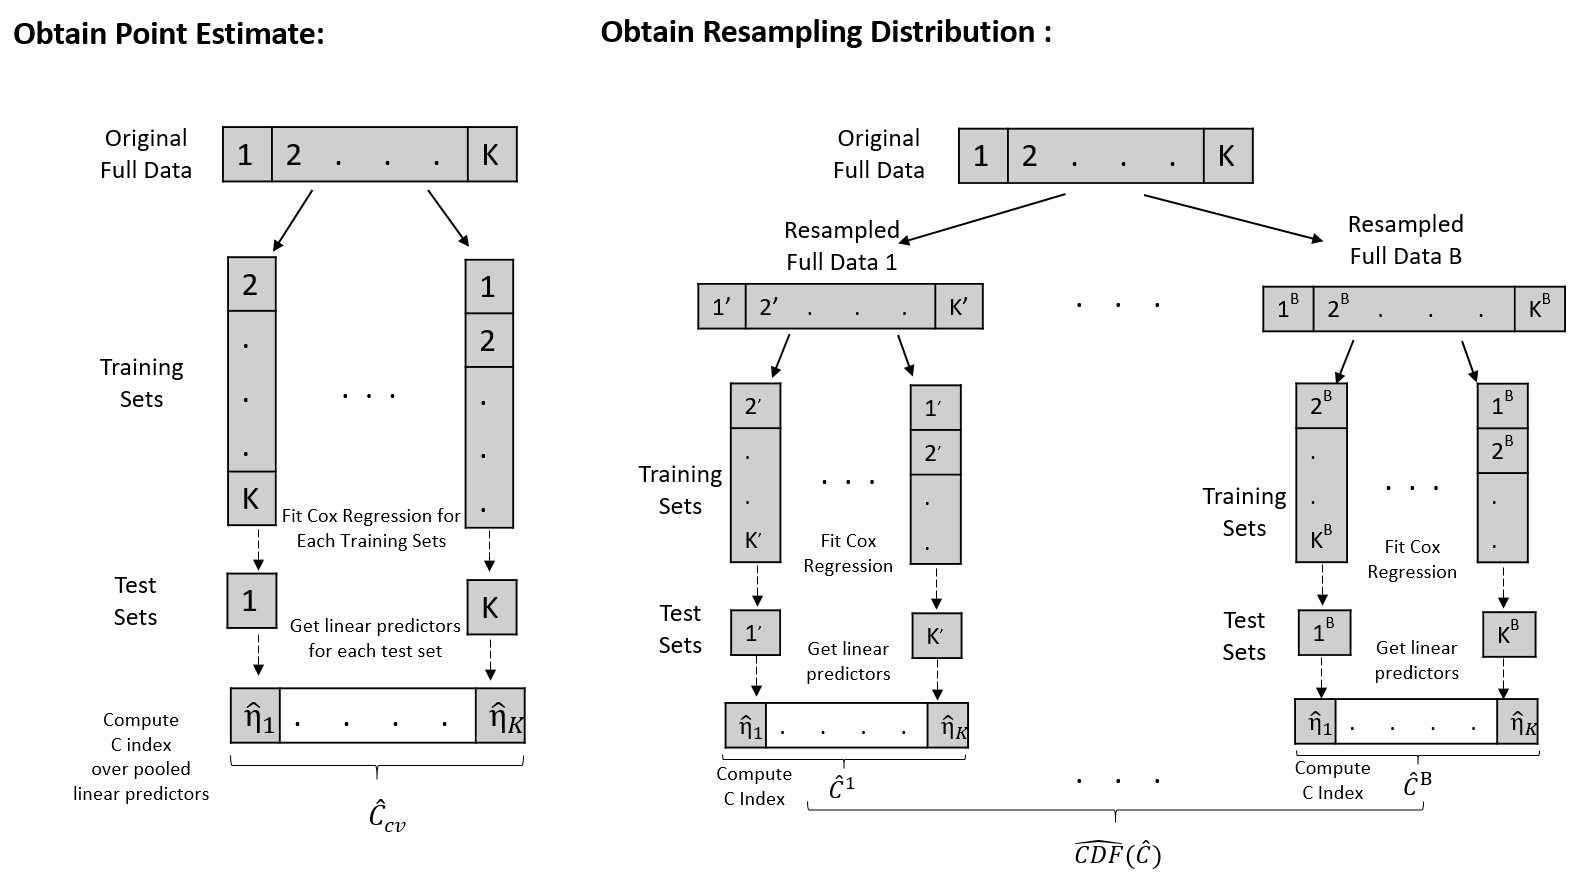
\includegraphics[width=16cm]{diagram.PNG}
	\end{figure}

%%%%%%%%%%%%%%%%%%%%%%%%%%%%%%%%%%
%%%%%%%%%%%%%%%%%%%%%%%%%%%%%%%%%%
%%%%%%%%%%%%%%%%%%%%%%%%%%%%%%%%%%

\section{Simulation Studies}
	
	\subsection{Data Generation and Simulation Design}
	
	\par Simulation studies were conducted under various scenarios to evaluate the operating characteristics of the proposed study design. Particularly, we are interested in the type one error rate, power and saving on sample size of the proposed study design.

	\par Assume there are p number of biomarkers for a study with sample size n, we can use $X_{n\times p}$ to denote the model matrix. We generate the biomarkers from independently and identically distributed normal distributions with mean 0 and standard error $\sigma$. The true prognostic signature is the true linear predictor $\eta = X\beta$, where $\beta$ is a vector of length p. For each biomarker, we can adjust their association with the outcome via the corresponding $\beta$ coefficient. 

	\par We assumed the actual survival time $T^0$ to be an exponential random variable. For each observation $i$, $T^{0}_{i}$ was generated from an exponential distribution with rate parameter $\lambda_{0}exp(\eta)$. Censoring status was generated under a right censoring mechanism described as follows. Censoring time $C$ was generated from independently identically distributed exponential distribution with rate parameter $\lambda_{c}$. The observed time $T$ and observed censoring status is defined as: 
	$$ (T,\delta)  = \begin{cases} 
					(T^{0}, 1), & \text{ if } T^{0} \leq C \\
					(C, 0), & \text{ if } T^{0} > C 
				   \end{cases} $$
One benefit of generating censoring status via two independent exponential distributions is that we can get the desirable event rate by tuning the ratio between $\lambda_{0}$ and $\lambda_{c}$. The probability of an event occurs is equal to the probability that the event time is less than or equal to the censoring time. Hence the event rate is equivalent to $Pr(T^0 - C \leq 0)$. Based on the probability distribution of $T^{0} - C$, which is the difference of two independent exponential random variables, we can get the the event rate exactly to be $\frac{\lambda_{0}}{\lambda_{0} + \lambda_{C}}$.

	\par The following scenarios were examined in our Monte Carlo simulation studies:
	\begin{itemize}
		\item Scenario 1: Hypothesis test of interest : $H_0: C \leq 0.5$ vs $H_1: C > 0.5 $.  To study type one error rate, we generated the covariate matrix and survival outcome independently, so that the true C is 0.5. To study power of our study design under this scenario, we generate the data sets where the true C statistic is 0.6 so that the alternative hypothesis is true. 
		\item Scenario 2: Hypothesis test of interest : $H_0: C \leq 0.6$ vs $H_1: C > 0.6 $. To study type one error rate, we generated data sets where the true C is 0.6 so that the null hypothesis is true. To study power of our design, we generate the data sets where the true C statistic is 0.65 and 0.7 so that the alternative hypothesis is true. 
	\end{itemize}

	\par Under each scenario, we varied expected event rates to be 30$\%$ and 70 $\%$, representing studies with higher censoring rate and studies with lower censoring rate. We set $\lambda_0$ to be 0.025. $\lambda_c$ was set to be $\frac{7}{3}\lambda_0$ to get 30$\%$ event rate; and $\frac{3}{7}\lambda_0$ to get 70$\%$ event rate. Overall sample size was varied to be $\left\{ 300, 500, 800 \right\}$ and the proportion of samples in first stage was varied to be S = $\left\{ 0.25, 0.5 , 0.75 \right\}$. The test levels for Stage 1 and Stage 2 were pre-specified at $\alpha_1 = 0.25$ and $\alpha_2 = 0.2$, so that the overall significance level of the design is set at $\alpha = \alpha_1 \times \alpha_2 = 0.05$. To avoid running into convergene issues for a Cox model, the rule of thumb is to have at least 10 events for each covariate. For each event rate, sample size, and split configuration, we used this rule of thumb to determine the number of biomarkers so that there are enough events for each biomarker in the smallest training set. 

	\par  The theoretical value of the C statistic is a function of the baseline hazard rate $\lambda_0$ and linear predictors $\eta = X\beta$, where X was generated from Normal$(0, \sigma^2)$. The true value of C can be seen as a point estimator of the proportion of concordance pairs, which is $Prob(\eta_{i} < \eta_{j} | T_{i} > T_{j})$ for all $i,j$ $\in \{1, ... , n \}$, assuming all events are observed. For some given values of $\lambda_0$, $\sigma$, and $\beta$, this probability can be computed via either numerical intergration or simulations based on large sample approximation. The latter was used in our data generating process to determine whether the desirable value of C was achieved for the parameters we used. 

	\par To compute the theoretical value of C, we generated two signature $\eta_{1}$ and $\eta_2$ and two corresponding times $T_{1}$ and $T_{2}$ in each iteration. This process will be repeated 10000 times. Among all 10000 pairs, we computed the proportion of pairs where $T_{1} > T_{2}$ and $\eta_{1} < \eta_{2}$ , or $T_{1} < T_{2}$ and $\eta_{1} > \eta_{2}$. We used this proportion as the true C value of the data set generated from some given parameters $\lambda_{0}$, $\sigma$, and $\beta$. 

	\par Since the true value of C can be affected by these three parameters, hence there are infinitely many combintations that generate a specific value of C, say 0.6. To simplify the data generating process, we fixed $\lambda_0 = 0.025$, $\sigma = log(1.5)$ and $p - 1$ elements of the $\beta$ vector and only varied one element in $\beta$ to achieve the desirable C statistic using the simulation procedure described above. One special case is when $\beta$ is set to 0 for all biomarkers. Then the actual survival times would no longer depend on the biomarkers, so that the expected C index would be 0.5.

	\par A total of N = 1000 iterations were run for the Monte Carlo simulations for each configuration in each scenario. Within each iteration, we recorded whether the null hypothesis is rejected. Under the null, the proportion of total number of hypothesis got rejected is the empirical estimate of the type one error rate. Under the alternative hypothesis, this is the empiricial estimate of power. Besides type one error rate and power, we also recorded the probabilility of early stopping and calculated expected sample size (E(SS)) and expected event size (E(ES)). Under the null, it is desirable to stop the study early and to reduce the cost of collecting more specimen. Under the alternative, it is desirable to have higher power to dectect a predictive signature. 

	\subsection{Simulation Results}

	\par Results of the simulation studies are presented in Table 1 and 2. Table 1 correspondes to Scenario 1, where the hypothesis of interest is $H_0: C \leq 0.5$ vs $H_1: C > 0.5$ and permutation test was used in Stage 1. Under the null hypothesis, the type one error rate is maintained around 0.05. Early stopping ranges from 72$\%$ to 78.5$\%$, which yields sample size reduction from 18 $\%$ to 40$\%$. Under the alternative hypothesis C = 0.6, the 50$\%$ vs 50$\%$ even split of sample always yields the highest power. With sufficient number of events, power can reach above $95\%$. We would expect power to be even better for greater improvement to the null.

	\par Results in Table 2 correspondes to Scenario 2, where the hypothesis of interest is at $C_0 = 0.6$. Bootstrapping was used in Stage 1 to conduct the early test. Under the null hypothesis, percentage of early stopping ranges from 74$\%$ to 80.9$\%$, yielding expected sample size reduction to be to 18.5$\%$ to 60$\%$. Under the alternative hypothesis C = 0.65, which is a small improvement to the null, power is generally low. Under the alternative hypothesis C = 0.7, which is a bigger and more meaningful improvement on the C index, the two stage design achieves 90 $\%$ power for all scenarios when the sample split is at 50$\%$ vs 50$\%$.
	
	\par Overall, our simulation study illustrated that the two stage adaptive design with permutation and bootstrap can keep type one error rate around pre-specified level and lead to significant sample size reduction when the prognostice signature is not predictive. Meanwhile, the two stage adaptive design has sufficient power to detect the true predictability of prognostic signatures.

%%%%%%%%%%%%%%%%%%%%%%%%%%%%%%%%%%
%%%%%          Insert table here                            %%%%%%%%%%
%%%%%%%%%%%%%%%%%%%%%%%%%%%%%%%%%%

	%%%%%%%%%%
%%% Table 1 %%%
%%%%%%%%%%

\begin{table}

\setlength{\tabcolsep}{3pt}

\caption{\label{tab:}Operating Characteristics of Two Stage Adaptive Design with Permutation}
\scriptsize
\centering
\begin{tabular}[t]{cccccccccccccc}
\toprule
 & & & & & & \multicolumn{4}{c}{Null Hypothesis: C = 0.5} & \multicolumn{4}{c}{Alternative Hypothesis: C = 0.6} \\ \cmidrule(lr){7-10} \cmidrule(lr){11-14}
N & Event & S & $n_1$ & $n_2$ & $\#\beta$ & $\%$Early & Type I & E(SS) & E(ES) & $\%$ Early& Power & E(SS) & E(ES)\\
 & Rate& & & & & Stop & Error & & &Stop & & &\\
\midrule
300 & 0.3 & 0.25 & 75 & 225 & 2 & 0.748 & 0.059 & 132 & 40 & 0.413 & 0.517 & 207 & 63\\
 &  & 0.50 & 150 & 150 & 2 & 0.732 & 0.064 & 190 & 57  & 0.192 & 0.712 & 271 & 83\\
 &  & 0.75 & 225 & 75 & 2 & 0.726 & 0.061 & 246 & 74  & 0.087 & 0.669 & 293 & 90\\
\addlinespace
500 & 0.3 & 0.25 & 125 & 375 & 4 & 0.728 & 0.089 & 227 & 68  & 0.334 & 0.617 & 375 & 115\\
 &  & 0.50 & 250 & 250 & 4 & 0.737 & 0.066 & 316 & 95  & 0.115 & 0.802 & 471 & 144\\
 &  & 0.75 & 375 & 125 & 4 & 0.729 & 0.062 & 409 & 123  & 0.043 & 0.782 & 495 & 151\\
\addlinespace
800 & 0.3 & 0.25 & 200 & 600 & 6 & 0.743 & 0.063 & 354 & 107  & 0.238 & 0.737 & 657 & 201\\
 &  & 0.50 & 400 & 400 & 6 & 0.756 & 0.051 & 498 & 150 &  0.049 & 0.928 & 780 & 239\\
 &  & 0.75 & 600 & 200 & 6 & 0.738 & 0.054 & 652 & 197 &  0.011 & 0.883 & 798 & 245\\
\addlinespace
300 & 0.7 & 0.25 & 75 & 225 & 5 & 0.733 & 0.059 & 135 & 94 &  0.258 & 0.707 & 242 & 168\\
 &  & 0.50 & 150 & 150 & 5 & 0.759 & 0.050 & 186 & 130 &  0.070 & 0.890 & 290 & 201\\
 &  & 0.75 & 225 & 75 & 5 & 0.745 & 0.054 & 244 & 170 &  0.015 & 0.859 & 299 & 207\\
\addlinespace
500 & 0.7 & 0.25 & 125 & 375 & 8 & 0.748 & 0.040 & 220 & 154  & 0.199 & 0.792 & 425 & 296\\
 &  & 0.50 & 250 & 250 & 8 & 0.785 & 0.043 & 304 & 213 & 0.017 & 0.978 & 496 & 344\\
 &  & 0.75 & 375 & 125 & 8 & 0.771 & 0.046 & 404 & 283 &  0.003 & 0.961 & 500 & 347\\
\addlinespace
800 & 0.7 & 0.25 & 200 & 600 & 10 & 0.739 & 0.049 & 357 & 250 &  0.053 & 0.947 & 768 & 534\\
 &  & 0.50 & 400 & 400 & 10 & 0.739 & 0.066 & 504 & 353 &  0.001 & 0.998 & 800 & 556\\
 &  & 0.75 & 600 & 200 & 10 & 0.726 & 0.064 & 655 & 459 &  0.000 & 0.992 & 800 & 556\\
\bottomrule
\end{tabular}
\end{table}

%%%%%%%%%%
%%% Table 2 %%%
%%%%%%%%%%
\begin{table}
\setlength{\tabcolsep}{2pt}
\caption{\label{tab:}Operating Characteristics of Two Stage Adaptive Design with Bootstrap}
\scriptsize
\centering
\begin{tabular}[t]{cccccccccccccccccc}
\toprule
 & & & & & & \multicolumn{4}{c}{Null Hypothesis: C = 0.6} & 
		\multicolumn{4}{c}{Alternative Hypothesis: C = 0.65} & 
		\multicolumn{4}{c}{Alternative Hypothesis: C = 0.7}\\ 
		\cmidrule(lr){7-10} 
		\cmidrule(lr){11-14}
		\cmidrule(lr){15-18}
N & Event & S & $n_1$ & $n_2$ & $\#\beta$ & $\%$Early & Type I & E(SS) & E(ES) & $\%$ Early& Power & E(SS) & E(ES)& $\%$ Early& Power & E(SS) & E(ES)\\
 & Rate& & & & & Stop & Error & & &Stop & & & & Stop & & &\\
\midrule
300 & 0.3 & 0.25 & 75 & 225 & 2 & 0.809 & 0.031 & 118 & 36 & 0.538 & 0.310 & 179 & 56 & 0.176 & 0.806 & 260 & 85\\
 &  & 0.50 & 150 & 150 & 2 & 0.800 & 0.048 & 180 & 55 & 0.365 & 0.407 & 245 & 77 & 0.044 & 0.915 & 293 & 95\\
 &  & 0.75 & 225 & 75 & 2 & 0.784 & 0.047 & 241 & 74 & 0.274 & 0.374 & 279 & 88 & 0.011 & 0.845 & 299 & 97\\
\addlinespace
500 & 0.3 & 0.25 & 125 & 375 & 4 & 0.771 & 0.025 & 211 & 64 & 0.379 & 0.451 & 358 & 112 & 0.066 & 0.927 & 475 & 154\\
 &  & 0.50 & 250 & 250 & 4 & 0.778 & 0.026 & 306 & 93 & 0.216 & 0.578 & 446 & 140 & 0.007 & 0.980 & 498 & 161\\
 &  & 0.75 & 375 & 125 & 4 & 0.780 & 0.042 & 402 & 123 & 0.130 & 0.523 & 484 & 152 & 0.000 & 0.931 & 500 & 162\\
\addlinespace
800 & 0.3 & 0.25 & 200 & 600 & 6 & 0.768 & 0.016 & 339 & 104 & 0.243 & 0.603 & 654 & 205 & 0.015 & 0.984 & 791 & 257\\
 &  & 0.50 & 400 & 400 & 6 & 0.768 & 0.029 & 493 & 151 & 0.104 & 0.718 & 758 & 238 & 0.000 & 0.999 & 800 & 260\\
 &  & 0.75 & 600 & 200 & 6 & 0.740 & 0.042 & 652 & 199 & 0.050 & 0.640 & 790 & 248 & 0.000 & 0.971 & 800 & 260\\
\addlinespace
300 & 0.7 & 0.25 & 75 & 225 & 5 & 0.752 & 0.012 & 131 & 91 & 0.306 & 0.511 & 231 & 159 & 0.051 & 0.940 & 289 & 195\\
 &  & 0.50 & 150 & 150 & 5 & 0.759 & 0.034 & 186 & 129 & 0.143 & 0.629 & 279 & 191 & 0.004 & 0.992 & 299 & 202\\
 &  & 0.75 & 225 & 75 & 5 & 0.774 & 0.046 & 242 & 168 & 0.081 & 0.579 & 294 & 202 & 0.000 & 0.951 & 300 & 203\\
\addlinespace
500 & 0.7 & 0.25 & 125 & 375 & 8 & 0.757 & 0.012 & 216 & 150 & 0.226 & 0.612 & 415 & 285 & 0.014 & 0.985 & 495 & 335\\
 &  & 0.50 & 250 & 250 & 8 & 0.808 & 0.019 & 298 & 207 & 0.081 & 0.792 & 480 & 330 & 0.000 & 0.999 & 500 & 338\\
 &  & 0.75 & 375 & 125 & 8 & 0.799 & 0.036 & 400 & 278 & 0.026 & 0.712 & 497 & 342 & 0.000 & 0.988 & 500 & 338\\
\addlinespace
800 & 0.7 & 0.25 & 200 & 600 & 10 & 0.748 & 0.019 & 351 & 244 & 0.096 & 0.823 & 742 & 511 & 0.000 & 1.000 & 800 & 541\\
 &  & 0.50 & 400 & 400 & 10 & 0.773 & 0.031 & 491 & 341 & 0.012 & 0.923 & 795 & 547 & 0.000 & 1.000 & 800 & 541\\
 &  & 0.75 & 600 & 200 & 10 & 0.775 & 0.042 & 645 & 448 & 0.003 & 0.834 & 799 & 550 & 0.000 & 1.000 & 800 & 541\\
\bottomrule
\end{tabular}
\end{table}


%%%%%%%%%%
%% Table 3 %%%%
%%%%%%%%%%
\begin{table}
\centering
\caption{\label{tab:}Locked Down Signature for Triple Negative Breast Cancer Dataset}
\begin{tabular}{lccc}
\toprule
 Biomarker & Estimate & Standard Error & p-value \\
\midrule
Age & 0.032 & 0.008 & $<$0.001\\
Stromal til & -0.012 & 0.005 & 0.014\\
Tumor size & 0.031 & 0.044 & 0.487\\
Ki67 & 0.004 & 0.004 & 0.281\\
Nodal status (1-3) & 0.753 & 0.261 & 0.004\\
Nodal status (4-9) & 1.171 & 0.337 & 0.001\\
Nodal status (10+) & 1.730 & 0.376 & $<$0.001\\
Chemotherapy (Adjuvant) & -0.520 & 0.343 & 0.130\\
Chemotherapy (Other) & -0.324 & 0.309 & 0.295\\
Chemotherapy (No) & 0.340 & 0.293 & 0.246\\
Radiotherapy(Yes vs No) & -0.223 & 0.211 & 0.291\\
NLR & 0.082 & 0.066 & 0.212\\
\bottomrule
\end{tabular}
\end{table}  % table.tex is in the same folder where manuscript.tex is

%%%%%%%%%%%%%%%%%%%%%%%%%%%%%%%%%%
%%%%%%%%%%%%%%%%%%%%%%%%%%%%%%%%%%
%%%%%%%%%%%%%%%%%%%%%%%%%%%%%%%%%%

\section{Example: Application to Real Dataset}
	\par We illustrated the proposed two-stage adaptive design with a real dataset of of early stage triple negative breast cancer (TNBC) patients. TNBC is an aggressive breast cancer subtype with substantial risk of disease recurrence. Recently, a retrospective study at Mayo Clinic demonstrated that percentage of Stromal TIL (sTIL), Ki67 and Neutrophil-to-lymphocyte ratio (NLR) are some additional prognostic biomarkers besides tumor size and nodal status \citep{Leon-Ferre2018}. 
	% Biyue needs more help here for TNBC background and data cleaning/imputation
	\par The study population is reviewed from a surgical cohort of 9982 patients who went through breast cancer surgery at Mayo Clinic between January 1985 and December 2012. 605 patientes were identified as TNBC. The outcome of interest is overall survival. The median follow-up for overall survival is 10.6 years (95$\%$ CI: 9.7 - 11.7). Among 605 patients, 223 events were observed. The event rate is about $36.86 \%$. We applied the two-stage adaptive design on this data set to build and validate a prognostic signature that consists of the following biomarkers: age, sTIL's, tumor size, Ki67, nodal status, adjuvant chemotherapy, adjuvant radiotherapy and NLR.

	\par We randomly split the data set into two stages with roughly equal sample size, stratified by patients' event status. Significance levels are specified at 0.25 and 0.2 respectively for the first and second stage. We wanted to demonstrate the two stage design in testing two null hypothesis: $H_0: C \leq 0.5$ and $H_0: C \leq 0.6$. For testing $H_0: C \leq 0.5$, permutation procedure is used in the first stage. For testing $H_0: C \leq 0.6$, bootstrap procedure is used in the first stage.

	\par In Stage 1, the point estimator of the cross-validated C index is 0.68. Permutation of 1000 iteration was carried out to estimate the null distribution around C = 0.5. The 75th percentile of the permutation distribution is 0.524, which leads to a rejection of $H_0: C \leq 0.5$ at $\alpha_1 = 0.25$ level. The study thus moves onto second stage. A locked-down pronostic signature was built based on all data in Stage 1. The final model is presented in Table 3. The C-index of applying the locked-down signature to Stage 2 data is 0.738. The standard error of the C index, estimated from Pencina's method, is 0.026. With normal approximation, the Z statistic from C = 0.5 is around 8.99. Hence we would reject the null hypothesis $H_0: C \leq 0.5$. And the prognostic signature is thus independently validated.

	\par For testing the hypothesis $H_0: C \leq 0.6$, bootstrap procedure with 1000 iteration was used in Stage 1. The 25th percentile of the bootstrap distribution is 0.676 , which is higher than $C_0 = 0.6$. Hence the null hypothesis $H_0 \leq 0.6$ would be rejected. The same locked-down signature in Table 3 would be used in the Stage 2. The Z statistic from C = 0.6 is around 5.22. Hence we would also reject the null hypothesis $H_0: C \leq 0.6$ and the prognostic signature is independently validated.

%%%%%%%%%%%%%%%%%%%%%%%%%%%%%%%%%%
%%%%%%%%%%%%%%%%%%%%%%%%%%%%%%%%%%
%%%%%%%%%%%%%%%%%%%%%%%%%%%%%%%%%%

\section{Discussion}
	% Biyue left the Discussion as bullet points so that it's easier for doing brainstorm
	\begin{itemize}
		\item alternative concordance measure (Harrell's C vs Uno's C, time-dependent AUC etc)
		\item definition of ties; bootstrap creates ties
		\item alternative testing statistics (association instead of discrimination)
		\item future extensions: higher dimension
		\item people may argue that for time-to-event outcome, the specimens may have already been collected by the time we analyze the data. then there is no actual sample size reduction or stopping for futility.
	\end{itemize}

\newpage
\bibliographystyle{unsrtnat}
\bibliography{reference}

\end{document}
